\begin{figure*}
	\center{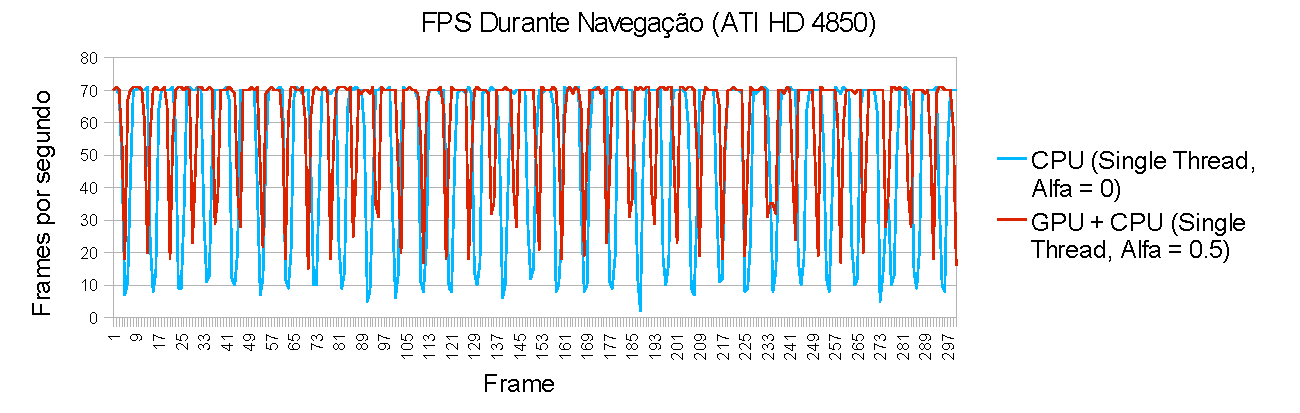
\includegraphics[width=0.8\linewidth]{img/fps_single.pdf}}
	\caption{\label{fig:fpssingle} Gr�fico com o FPS na navega��o pelo mundo durante 300 segundos, utilizando uma �nica \emph{thread} na CPU.}
\end{figure*}

\begin{figure*}
	\center{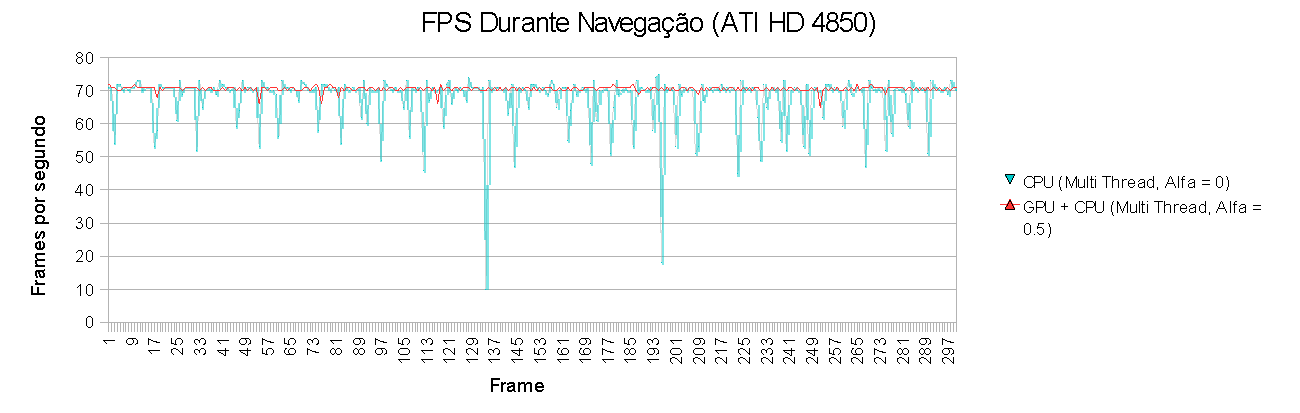
\includegraphics[width=0.8\linewidth]{img/fps_multi.pdf}}
	\caption{\label{fig:fpsmulti} Gr�fico com o FPS na navega��o pelo mundo durante 300 segundos, utilizando m�ltiplas \emph{threads} na CPU.}
\end{figure*}

%\begin{figure*}[t]
%	\center{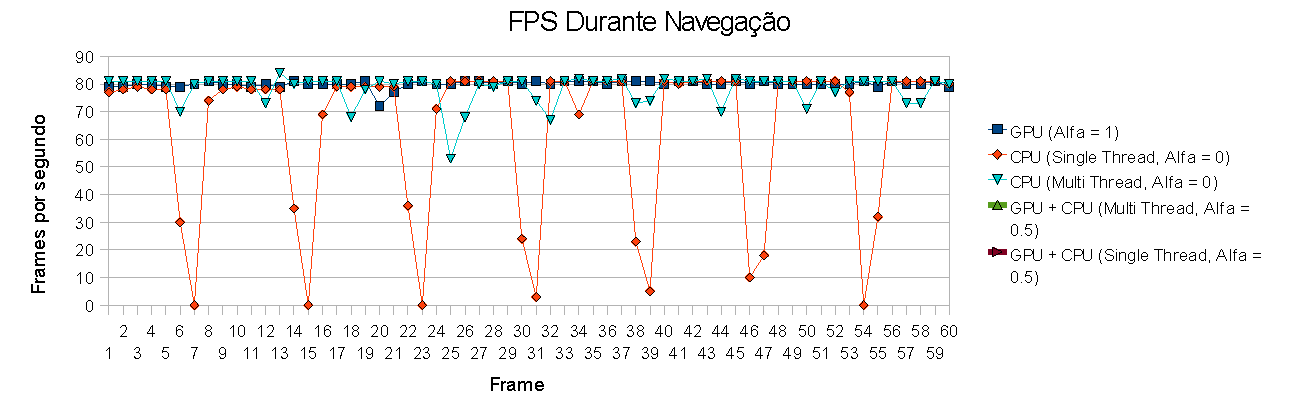
\includegraphics[width=1.0\linewidth]{img/fps.pdf}}
%	\caption{\label{fig:fps} Gr�fico com o FPS na navega��o pelo mundo durante 60 segundos.}
%\end{figure*}

%\begin{figure}[h]
%	\center{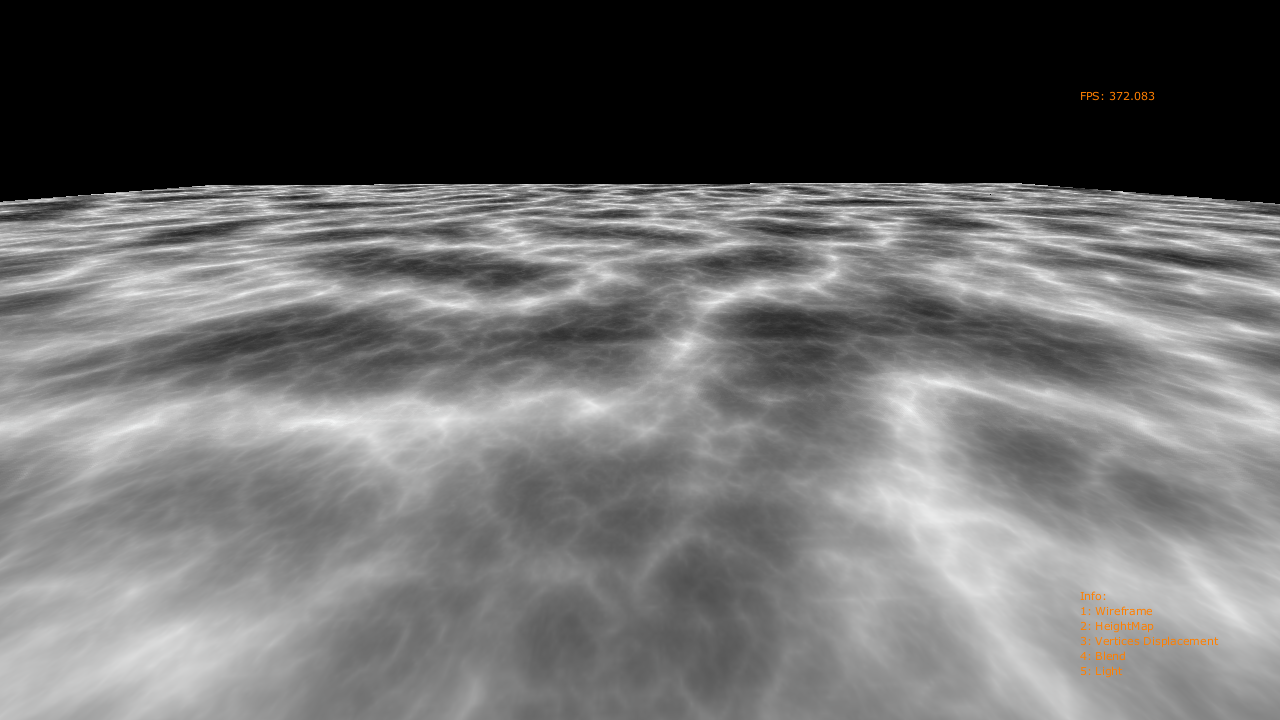
\includegraphics[width=1.0\linewidth]{img/caps/heightmap.png}}
%	\caption{\label{fig:heightmap} Mapa de altura aplicado a um quadrado.}
%\end{figure}

%\begin{figure}[h]
%	\center{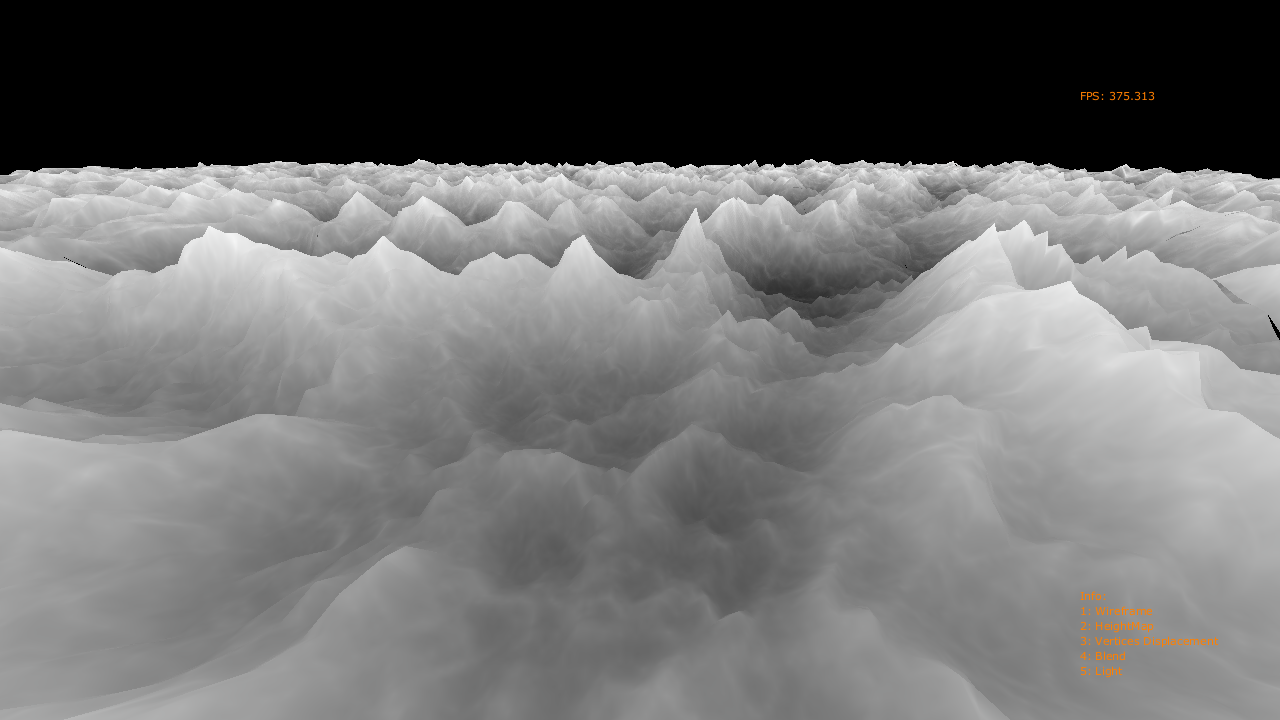
\includegraphics[width=1.0\linewidth]{img/caps/deslocamento.png}}
%	\caption{\label{fig:deslocamento} Mapa de altura aplicado a um quadrado, deslocando a altura.}
%\end{figure}

%\begin{figure}[h]
%	\center{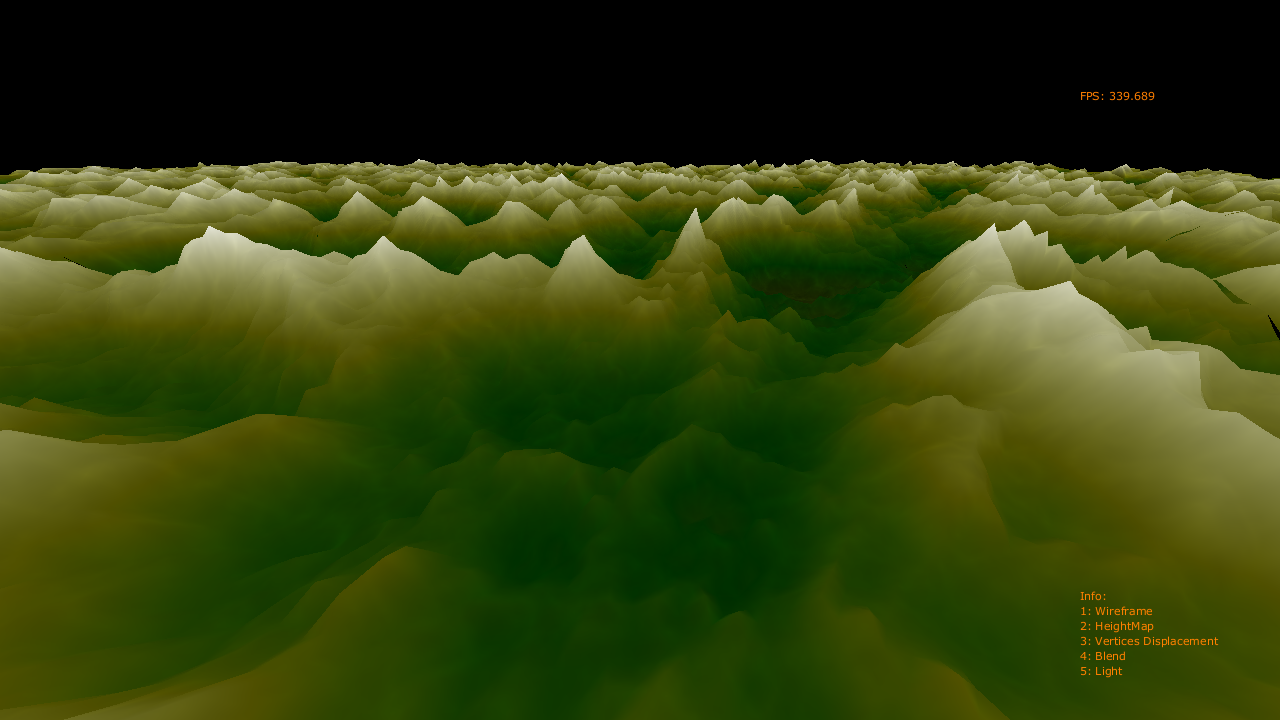
\includegraphics[width=1.0\linewidth]{img/caps/blend.png}}
%	\caption{\label{fig:blend} Mapa de altura aplicado a um quadrado, deslocando a altura, e com texturas.}
%\end{figure}

%\begin{figure}[h]
%	\center{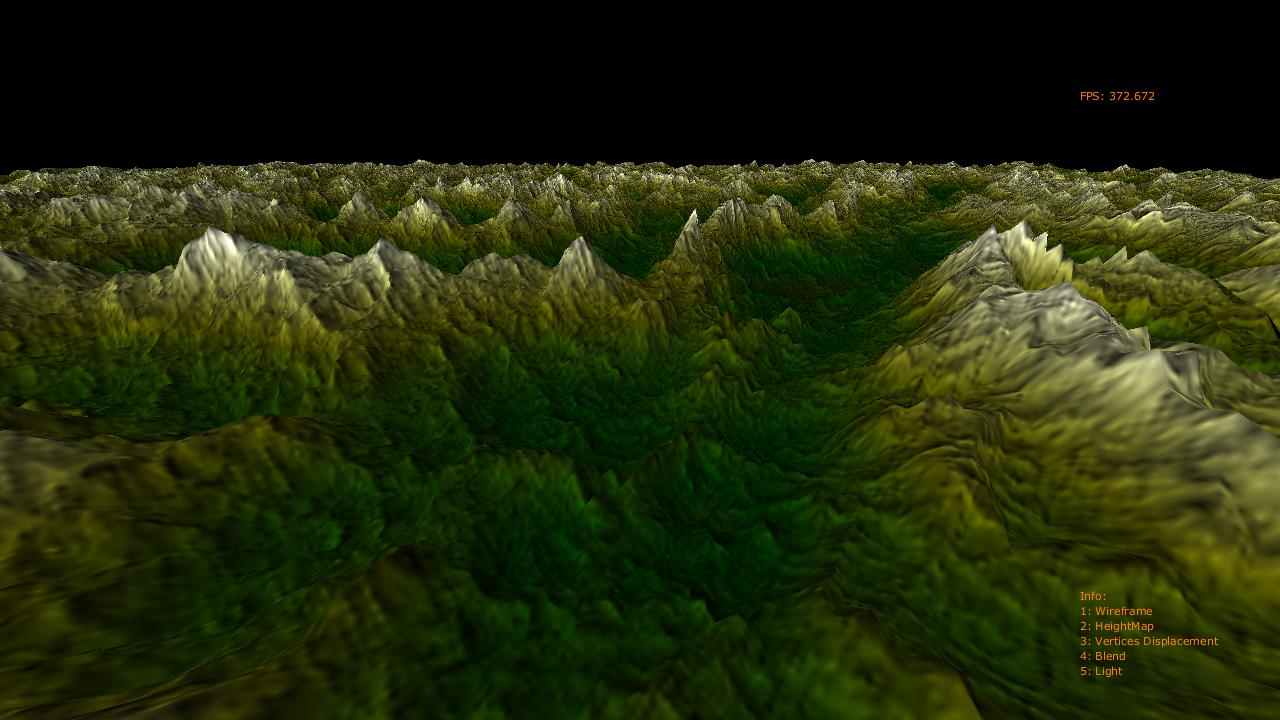
\includegraphics[width=1.0\linewidth]{img/caps/luz.png}}
%	\caption{\label{fig:luz} Mapa de altura aplicado a um quadrado, deslocando a altura, com texturas, e %ilumina��o.}
%\end{figure}